\documentclass{standalone}

\usepackage{tikz}
\usetikzlibrary{math}

\begin{document}
    Pascal Triangle or Yanghui Triangle.
    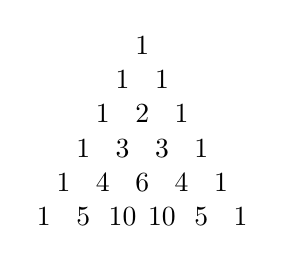
\begin{tikzpicture}
        \foreach \ja in {0,...,5}
        {
            \foreach \jb in {0,...,\ja}
            {
                \tikzmath {
                    int \aaaaa;
                    \aaaaa = ((\ja)!)/((\jb)! * (\ja - \jb)!);
                };
                \node at (
                    {((-1) * \ja * (0.5)*(0.5))+(2*\jb * (0.5)*(0.5))},
                    {(-1)*\ja *(sqrt(3)/2)*(0.5)}
                ){\aaaaa};
            }
        }
    \end{tikzpicture}
\end{document}